\subsubsection{Package della componente ViewModel}
	\begin{center}
		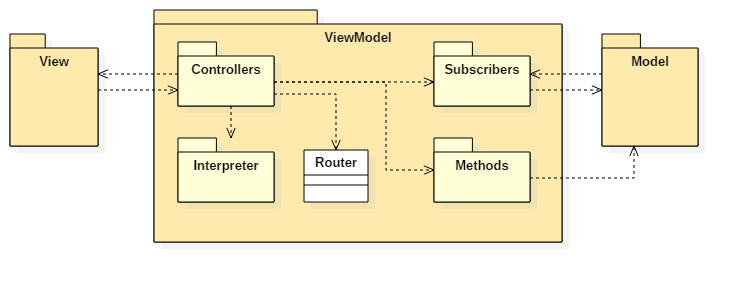
\includegraphics[scale=0.65]{../images/ViewModelPackage.png}
	\end{center}
	Gli elementi del package collaborano e interagiscono con l'obiettivo comune di realizzare il data-binding con i componenti della View e interagire col Model per richiedere e aggiornare i dati.
	Il package del ViewModel contiene i seguenti sub-packages:
	\begin{itemize}
	\item \textbf{Controllers}: Il package contiene tutti i \emph{Controller} del sistema Quizzipedia. Ogni \emph{Controller} implementa le funzionalità associate ad un template della View.
	Il package contiene al suo interno le classi:
	\begin{itemize}
		\item \textit{NewQuestionController}
		\item \textit{NewQuizController}
		\item \textit{QuizManagementController}
		\item \textit{QuizListController}
		\item \textit{QuizDetailsController}
		\item \textit{DeleteQuestionController}
		\item \textit{DeleteQuizController}
		\item \textit{QuestionsManagementController}
		\item \textit{QMLEditorController}
	\end{itemize}	
	
	\item \textbf{Subscribers}: Il package contiene le classi necessarie ad effettuare il \emph{subscribing} delle collezioni di dati pubblicate dal \emph{server}.
	Il package contiene al suo interno le classi:
	\begin{itemize}
		\item \textit{QuestionsSubscriber}
		\item \textit{QuizSubscriber}
		\item \textit{UsersSubscriber}
	\end{itemize}
	
	\item \textbf{Methods}: Il package contiene le classi necessarie all'utilizzo dei \emph{Methods} di Meteor nel sistema, che permettono al \emph{client} di richiedere modifiche ai dati al \emph{server}.
	Il package contiene al suo interno le classi:
	\begin{itemize}
		\item \textit{QuestionMethods}
		\item \textit{QuizMethods}
		\item \textit{UserMethods}
	\end{itemize}		
	
	\item \textbf{Interpreter}:
	Il package \emph{Interpreter} è responsabile della traduzione di testo QML in codice HTML5 visualizzabile da browser. Per permettere al package di essere estendibile in futuro con nuovi tipi di "Interpreter", le classi al suo interno sono organizzate seguendo il pattern \emph{Abstract Factory} . \\
	Il package contiene al suo interno le seguenti classi:
	\begin{itemize}
	\item \textit{Interpreter}
	\item \textit{InterpreterFactory}
	\item \textit{QMLInterpreterFactory}
	\item \textit{QMLInterpreter}
	\item \textit{QML2HTMLInterpreter}
	\end{itemize}
		
	\item \textbf{Router}:
Il package implementa il routing e la visualizzazione dinamica dei template dei sistema, fornendo ad una single-page application le caratteristiche tipiche di un sistema web server-side. Contiene la classe:
\begin{itemize}
	\item\textit{Router}
\end{itemize}
\end{itemize}

\newpage